\documentclass[12pt]{report}
\usepackage{%
	amsfonts,%
	amsmath,%	
	amssymb,%
	amsthm,%
	algorithm,%
	babel,%
	bbm,%
	etex,%
	%biblatex,%
	caption,%
	centernot,%
	color,%
	dsfont,%
	enumerate,%
	epsfig,%
	epstopdf,%
	geometry,%
	graphicx,%
	hyperref,%
	latexsym,%
	mathtools,%
	multicol,%
	pgf,%
	pgfplots,%
	pgfplotstable,%
	pgfpages,%
	proof,%
	psfrag,%
	subfigure,%	
	tikz,%
	ulem,%
	url%
}	
\usepackage[noend]{algpseudocode}
\usepackage[mathscr]{eucal}
\usepgflibrary{shapes}
\usetikzlibrary{%
  	arrows,%
	backgrounds,%
	chains,%
	decorations.pathmorphing,% /pgf/decoration/random steps | erste Graphik
	decorations.text,%
	matrix,%
  	positioning,% wg. " of "
  	fit,%
	patterns,%
  	petri,%
	plotmarks,%
  	scopes,%
	shadows,%
  	shapes.misc,% wg. rounded rectangle
  	shapes.arrows,%
	shapes.callouts,%
  	shapes%
}

\theoremstyle{plain}
\newtheorem{thm}{Theorem}[section]
\newtheorem{lem}[thm]{Lemma}
\newtheorem{prop}[thm]{Proposition}
\newtheorem{cor}[thm]{Corollary}

\theoremstyle{definition}
\newtheorem{defn}[thm]{Definition}
\newtheorem{conj}[thm]{Conjecture}
\newtheorem{exmp}[thm]{Example}
\newtheorem{assum}[thm]{Assumptions}
\newtheorem{axiom}[thm]{Axiom}

\theoremstyle{remark}
\newtheorem{rem}{Remark}
\newtheorem{note}{Note}
\newtheorem{fact}{Fact}

\newcommand{\norm}[1]{\left\lVert#1\right\rVert}
\newcommand{\indep}{\!\perp\!\!\!\perp}
\DeclarePairedDelimiter\abs{\lvert}{\rvert}%
\newcommand\numberthis{\addtocounter{equation}{1}\tag{\theequation}}
\newcommand{\tr}{\operatorname{tr}}
\newcommand{\R}{\mathbb{R}}
\newcommand{\N}{\mathbb{N}}
\newcommand{\E}{\mathbb{E}}
\newcommand{\Z}{\mathbb{Z}}
\newcommand{\B}{\mathscr{B}}
\newcommand{\C}{\mathcal{C}}
\newcommand{\T}{\mathscr{T}}
\newcommand{\F}{\mathcal{F}}
\newcommand{\G}{\mathcal{G}}
%\newcommand{\ba}{\begin{align*}}
%\newcommand{\ea}{\end{align*}}
\DeclareMathOperator*{\argmax}{arg\,max}
\renewcommand{\qedsymbol}{$\blacksquare$}
\makeatletter
\def\BState{\State\hskip-\ALG@thistlm}
\makeatother

\makeatletter
\def\th@plain{%
  \thm@notefont{}% same as heading font
  \itshape % body font
}
\def\th@definition{%
  \thm@notefont{}% same as heading font
  \normalfont % body font
}
\makeatother
\date{}
\usepackage{scribe_e1244}
%\usepackage{graphicx}
%\newcommand{\E}{\mathbb{E}}
\begin{document}
\lecturer{Parimal parag}	
\scribe{P Shiva Kumar \& K Vikas Bharadwaj}
\lecturenumber{10}
\lecturedate{February 7}
\maketitle
%\newtheorem{rmk}{Remark}
%\newtheorem{exmp}{Example}[section]
% title of the lecture
\begin{center}
	{\Large \bf SIGNAL DETECTION IN DISCRETE TIME}
\end{center}
\section{Recap}
	We have studied optimum detector structures for coherent symbols in discrete time in presence of i.i.d gaussian noise and i.i.d laplacian noise. We also studied locally optimum detection of coherent symbols in i.i.d gaussian and laplacian noises where we assumed that the form of signal detected is known but not its amplitude.  
\section{Deterministic signal detection in gaussian dependent noise}
The basic problem that we are dealing is the following hypothesis testing problem:
\begin{center}
	$H_0 : \bar{Y}  = \bar{S_0}+ \bar{N}$
\end{center}
\begin{center}
 	$ H_1 :\bar{Y} = \bar{S_1}+ \bar{N}$
 \end{center}
    where  
    \begin{center}
    	$\bar{Y}=[Y_1\quad  Y_2\dots Y_n ]^T$ 
    \end{center} is a vector in the observation space, $\mathcal{R}^n$,
    \begin{center}
    $\bar{S_0}=[s_{01}\quad  s_{02}\dots s_{0n} ]^T$ 
    \end{center}
    \begin{center}
    	 $\bar{S_1}=[s_{11}\quad  s_{12}\dots s_{1n} ]^T$
    \end{center}
are the two deterministic and known signals, in discrete time and
   
   	\begin{center}
   		 $\bar{N}=[N_1\quad  N_2\dots N_n ]^T$
   	\end{center}
   is the vector of noise samples that are added to the signals and is gaussian with zero mean and covariance matrix $\varSigma_{N}$, i.e., $\E\lbrace\bar{N}\bar{N}^T\rbrace= \varSigma_{N}$
   \\The likelihood ratio corresponding to an observation $\bar{y}$ is given by 
   \[L(\bar{y})=\frac{\E_1\lbrack p_N(\bar{y}-\bar{S_1})\rbrack}{\E_0\lbrack p_N(\bar{y}-\bar{S_0})\rbrack}\]
  \begin{rmk} $\E_i$ denotes expectation over $\bar{S_i}$ for $i=\{0,1\}$ and $p_{\bar{N}}(x)$ denotes the probability density function of $\bar{N}$ at a vector $x$.\end{rmk}
Since the signals $\bar{S_0}$ and $\bar{S_1}$ are deterministic, the likelihood ratio simplifies to 
 
   \begin{equation}  
\label{eq1}L(\bar{y})=\frac{ p_{\bar{N}}(\bar{y}-\bar{S_1})}{ p_{\bar{N}}(\bar{y}-\bar{S_0})}
\end{equation}
For a gaussian vector $\bar{X}$ with mean $\bar{\mu}$ and covariance matrix $\varSigma_{N}$, its probability density function is given by 
  \[p_{\bar{X}}(x)= {\frac{1}{(2\pi)^{n/2}det(\varSigma_{N}))^{1/2}}}{exp\lbrack-{\frac{1}{2}}{(\bar{X}-\bar{\mu})^T}{{\varSigma_{N}}^{-1}}{(\bar{X}-\bar{\mu})}\rbrack}\]
  Then the likelihood ratio in $\eqref{eq1}$ becomes
  
\begin{align*}L(\bar{y})&=\frac{{\frac{1}{(2\pi)^{n/2}det(\varSigma_{N}))^{1/2}}}{exp\lbrack-{\frac{1}{2}}{(\bar{y}-\bar{S_1})^T}{{\varSigma_{N}}^{-1}}{(\bar{y}-\bar{S_1})}\rbrack}}{{\frac{1}{(2\pi)^{n/2}det(\varSigma_{N}))^{1/2}}}{exp\lbrack-{\frac{1}{2}}{(\bar{y}-\bar{S_0})^T}{{\varSigma_{N}}^{-1}}{(\bar{y}-\bar{S_0})}\rbrack}}\\& =exp{\lbrack{\frac{1}{2}}{(\bar{y}-\bar{S_0})^T}{{\varSigma_{N}}^{-1}}{(\bar{y}-\bar{S_0})}-{\frac{1}{2}}{(\bar{y}-\bar{S_1})^T}{{\varSigma_{N}}^{-1}}{(\bar{y}-\bar{S_1})}\rbrack}\\& =exp{\lbrack{\bar{S_1}^T{\varSigma_{N}}^{-1}{\bar{y}}-\bar{S_0}^T{\varSigma_{N}}^{-1}{\bar{y}}-{\frac{1}{2}}\bar{S_1}^T{\varSigma_{N}}^{-1}{\bar{S_1}}+{\frac{1}{2}}\bar{S_0}^T{\varSigma_{N}}^{-1}{\bar{S_0}}\rbrack}}\\& =exp{\lbrack{(\bar{S_1}-\bar{S_0})^T{\varSigma_{N}^{-1}({\bar{y}-\frac{\bar{S_0}+\bar{S_1}}{2}})}\rbrack}}\end{align*}
\noindent Upon taking natural logarithm, we have

 \[\ln(L(\bar{y}))=(\bar{S_1}-\bar{S_0})^T{\varSigma_{N}^{-1}}({\bar{y}-\frac{\bar{S_0}+\bar{S_1}}{2}})\]
 
 
 \[\Rightarrow\quad\ln(L(\bar{y}))=(\bar{S_1}-\bar{S_0})^T{\varSigma_{N}^{-1}}{\bar{y}}-{\frac{(\bar{S_1}-\bar{S_0})^T{\varSigma_{N}^{-1}}(\bar{S_0}+\bar{S_1})}{2}}\]\noindent Now by defining $\tilde{S}^T:=(\bar{S_1}-\bar{S_0})^T{\varSigma_{N}^{-1}}$, it can be seen that $T(\bar{Y}) \triangleq \tilde{S}^T\bar{Y}$ is a linear transformation of the gaussian random vector $\bar{Y}$ and hence the decision rule is given by
\begin{equation}
\label{eq2}\tilde{\delta}_0 (\bar{y})=
\begin{cases}
1 &if \quad\tilde{S}^T\bar{y}>\tau''   \\
\gamma &if\quad\tilde{S}^T\bar{y}= \tau''\\
0 &if\quad\tilde{S}^T\bar{y} <\tau''\\
\end{cases}
\end{equation}
where
\[\tau''=\ln(\tau)+{\frac{(\bar{S_1}-\bar{S_0})^T\varSigma_{N}^{-1}(\bar{S_0}+\bar{S_1})}{2}}\]
The structure of the detector is similar to that of a correlation detector is shown below.
\begin{figure}
	\begin{center}
	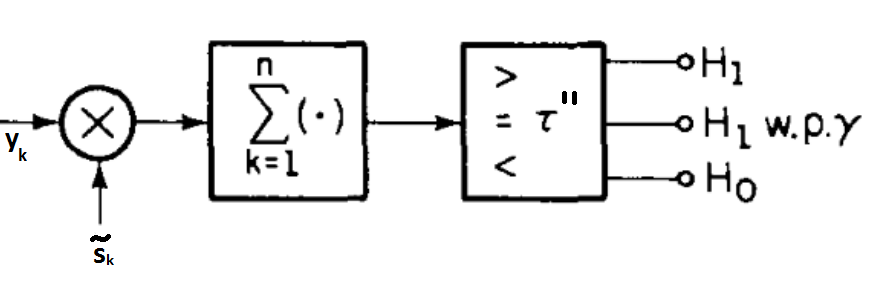
\includegraphics[scale=0.7]{figures/Lec10-fig1.png}
	\caption{Implementation of detector in \eqref{eq2}}
\end{center}
\end{figure}\\
\indent A property of multivariate gaussian distributions is that their linear transformations are also gaussian. Hence $T(\bar{Y})$ is a gaussian random variable and thus, we can characterize its distribution under $H_0$ and $H_1$ completely by finding its mean and variance under the two hypotheses.\\\indent Under $H_j$ the mean of $T(\bar{Y})$ is given by
\begin{align*}
 \E\lbrace T(\bar{Y})|H_j\rbrace &=\E\lbrace \tilde{S}^T\bar{Y}|H_j\rbrace\\&=\tilde{S}^T\E\lbrace\bar{Y}|H_j\rbrace\\&=\tilde{S}^T\bar{S_j}\triangleq\tilde\mu_j
\end{align*}
  Similarly, the variance of $T(\bar{Y})$ under $H_j$ is 
  \begin{align*}
  Var(T(\bar{Y})|H_j)&=\E\lbrace(\tilde{S}^T(\bar{Y}-\bar{S_j}))^2|H_j\rbrace\\&=\E\lbrace(\tilde{S}^T\bar{N})^2|H_j\rbrace\\&=\E\lbrace(\tilde{S}^T\bar{N})^2\rbrace\\&=\E\lbrace\tilde{S}^T\bar{N}\bar{N}^T\tilde{S}\rbrace
\\&=\tilde{S}^T\varSigma_{N}\tilde{S}\\&= (\bar{S_1}-\bar{S_0})^T{\varSigma_{N}^{-1}}(\bar{S_1}-\bar{S_0})=:d^2 \end{align*}
  Note that the variance of $T(\bar{Y})$ is independent of the hypotheses. Also note that positive definiteness of $\varSigma_{N}$ imples positive definiteness of $\varSigma_{N}^{-1}$ and thus that $d^2>0$ unless $\bar{S_0}=\bar{S_1}$.
  
 From the analysis above, we see that $T(\bar{Y})\sim\mathcal{N}(\tilde{S}^T\bar{S_j},d^2)$ under $H_j$ for $j=0,1$ and $ {\Gamma }_{1} $ can be formulated as,
\begin{center}
$ {\Gamma }_{1}= \lbrace \bar{y} : T(\bar{y})>\tau''\rbrace $
\end{center}
See that the randomized partition of $\Gamma$ in eqn$\eqref{eq2}$ is irrelevant because of the continuity of $T(\bar{y})$. The probability of deciding $H_1$ under $H_j$ is thus given by 
\begin{align*}
p_j(\Gamma_1)&=\underset{\Gamma_1 }{\int }\frac{1}{\sqrt{2\pi {d}^{2}}}{exp(-\frac{(\bar{y}-\tilde{S}^T\bar{S_j})^2}{2d^2})}d\bar{y}\\ &=1-\mathbf{\Phi}(\frac{\tau''-\tilde{S}^T\bar{S_j}}{d})
\end{align*}
where $\mathbf{\Phi}(.)$ is the standard normal distribution function.
Upon substituting $\tau''$ in $p_j(\Gamma_1)$, we have
\[ p_j(\Gamma_1)=
\begin{cases}
1-\mathbf{\Phi}(\frac{\ln\tau}{d}+\frac{d}{2}) &if\quad j=0 \\
1-\mathbf{\Phi}(\frac{\ln\tau}{d}-\frac{d}{2}) &if\quad j=1
\end{cases} \]
Then we can have expressions for detection probability and false alarm probability. 
\begin{exmp}For an $\alpha$-level Neyman Pearson testing we set,$\alpha=p_F(\tilde{\delta}_0)=p_0(\Gamma_1)$\\ \\ \indent \indent
$i.e.,\alpha=1-\mathbf{\Phi}(\frac{\tau''-\tilde{\mu}_0}{d})$\\ \\ \indent \indent $\Rightarrow\tau''=d\mathbf{\Phi}^{-1}(1-\alpha)+\tilde{\mu}_0$ \\now, the corresponding detection probablity becomes
\begin{align*}
p_1(\Gamma_1)&=1-\mathbf{\Phi}(\frac{\tau''-\tilde{\mu}_1}{d})\\ &=1=\mathbf{\Phi}(\frac{d\mathbf{\Phi}^{-1}(1-\alpha)+\tilde{\mu}_0-\tilde{\mu}_1}{d})\\&=1-\mathbf{\Phi}(\mathbf{\Phi}^{-1}(1-\alpha)+\frac{\tilde{\mu}_0-\tilde{\mu}_1}{d})
\end{align*}
\begin{align*}
\frac{\tilde{\mu}_0-\tilde{\mu}_1}{d}&=\frac{\tilde{S}^T(\bar{S_0}-\bar{S_1})}{d}\\&=\frac{(\bar{S_1}-\bar{S_0})^T\varSigma_N^{-1}(\bar{S_0}-\bar{S_1})}{d}\\&=\frac{-d^2}{d}\\&=-d
\end{align*}
\[\Rightarrow p_1(\Gamma_1)=p_D(\tilde{\delta}_{NP})=1-\mathbf{\Phi}(\mathbf{\Phi}^{-1}(1-\alpha)-d)\]\end{exmp}
\section{Interpretation of $\mathbf{d^2}$:}
In view of the discussion above we see that the performance of optimum detection of deterministic signals in gaussian noise improves monotonically with increasing d.This quantity (or more properly its square)can be interpretaed as a measure of signal-to-noise ratio. To see this, consider, without loss of generality,
signals $\bar{S_0}=\bar{0},\bar{S_1}=\bar{s}$. The noise samples can be independent or dependent.
\subsection{I.I.D noise} $\bar{N}$ is a zero mean gaussian random vector with covariance matrix $\varSigma_N =\sigma^2I $, where $I$ denotes the $n\times n$ identity matrix.\\Therefore,  $\varSigma_N^{-1}= \frac{1}{\sigma^2}I$. Hence
\begin{align*}d^2&=(\bar{S_1}-\bar{S_0})^T\varSigma_{N}^{-1}(\bar{S_1}-\bar{S_0})\\&=\frac{(\bar{S_1}-\bar{S_0})^T(\bar{S_1}-\bar{S_0})}{\sigma^2}\\&=\sum_{k=1}^{n}\frac{(s_1-s_0)^2_k}{\sigma^2}\\&=\frac{1}{\sigma^2}\sum_{k=1}^{n}(s_1-s_0)^2_k\end{align*}  upon substituting  $\bar{S_0}=\bar{0},\bar{S_1}=\bar{s}$,we get \\
\begin{align*}
d^2&=\frac{1}{\sigma^2}\sum_{k=1}^{n}s^2_k\\ &=n\frac{\bar{s^2}}{\sigma^2}
\end{align*}
here $\bar{s^2}$: is the Average signal power and  \\ \indent $\sigma^2$: is the Average noise power,  mathematically formulated as,\\ \\
\indent $\bar{s^2}\triangleq\frac{1}{n}\sum_{k=1}^{n}s^2_k $\\ \\
\indent $\sigma^2\triangleq\frac{1}{n}\sum_{k=1}^{n}\E{N^2_k}$
\\Therefore $d^2$ here is given by the average signal-to-noise ratio times the number of samples. Thus performance is enhanced by increasing either of these quantities, and as either of the two increases without bound perfect performance can result.
\subsection{Non-i.i.d noise} A similar interpretation can be given to $d^2$ in the non-i.i.d. case where $\bar{N}$ is a zero mean gaussian random vector with covariance matrix $\varSigma_{N}$.We can write the quantity $\sum_{k=1}^{n}\tilde{S}_ky_k $ as the input at time $n$ of a linear time-invariant filter with impulse response
\[\tilde{h}_k=\begin{cases}
\tilde{S}_{n-k} &for \quad0\leq k \leq n-1\\ 0 &otherwise
\end{cases}\]
\begin{figure}
	\begin{center}
		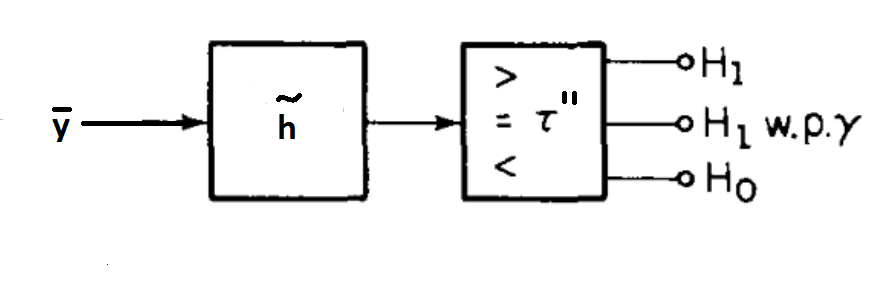
\includegraphics[scale=0.7]{figures/Lec10-fig2.png}\caption{Implementation of detector in the form of an LTI filter}
	\end{center}
\end{figure}
If the input to this filter is $\bar{s}= (s_1\dots s_n)$,then the output at time $n$ would be
\begin{align*}
\sum_{k=1}^{n}\tilde{S}_ks_k&= \bar{s}^T\varSigma_{N}^{-1}\bar{s}\\&= d^2
\end{align*}
Thus the output power at the sampling time due to signal only is $d^4$. On the other hand, if the noise only were put into this filter, the output at time $n$ would be $\sum_{k=1}^{n}\tilde{S}_kN_k $ a random quantity with variance
\begin{align*}
\E(\sum_{k=1}^{n}\tilde{S}_kN_k)^2&=\E({\bar{\tilde{S}}}^T\bar{N})^2\\ &=\bar{\tilde{S}}^T\varSigma_{N}\bar{\tilde{S}}\\ &=\bar{s}^T\varSigma_{N}^{-1}\varSigma_{N}\varSigma_{N}^{-1}\bar{s}\\ &=\bar{s}^T\varSigma_{N}^{-1}\bar{s}\\ &= d^2
\end{align*}
The ratio of signal power to noise variance at the output of filter at each sampling instant is
\begin{align*}
\frac{(\sum_{k=1}^{n}\tilde{S}_ks_k)^2}{\mathbb{E}\lbrace( \sum_{k=1}^{n}\tilde{S}_kN_k)^2\rbrace}&= \frac{d^4}{d^2}\\&=d^2
\end{align*}
Thus the quantity $d^2$ in the general case is the signal-to-noise power ratio at the output of the filter used for optimum detection at the sampling time $n$.It is intuitively reasonable that the higher this output SNR is, the better the signal can be detected by comparing the sampled output to a threshold, and this intuition is borne out by the monotonicity of detection of performance as a function of $d^2$ shown above.\\
The quantity $d^2$ also has another interpretation for the i.i.d. case with general signals $\bar{S_1},\bar{S_0}$\\
\[\bar{N}\sim i.i.d\quad and \quad \bar{N}\sim\mathcal{N}(\bar{0},\sigma^2I)\]
in this case, we can write $d^2=\frac{\parallel\bar{S_1}-\bar{S_0}\parallel^2}{\sigma^2}$,
where $\parallel\bar{S_1}-\bar{S_0}\parallel$ denotes the Euclidean distance between the signal vectors $\bar{S_0}$ and $\bar{S_1}$ given by
\[{\parallel\bar{S_1}-\bar{S_0}\parallel}_2={\lbrack{\sum_{k=1}^{n}(s_{1k}-s_{0k})^2}\rbrack}^{1/2}\]
Thus the farther apart the signal vectors are, the better performance can be achieved. A similar interpretation can be made for non-i.i.d. noise case also.
 
\section{Reduction to the i.i.d. noise case:}
 Since $\varSigma_{N}$ is positive definite, it can be written as   
 \begin{center}
$ \varSigma_{N}=CC^T$
 \end{center} where $C$ is an $n\times n$ invertible lower triangular matrix and also above form of $\varSigma_{N}$ is called the \textit{Cholesky decomposition} of $\varSigma_{N}$ and there are several standard algorithms for finding $C$ from $\varSigma_{N}$. We can write,
\begin{align*}
\varSigma_{N}^{-1}&=(CC^T)^{-1}\\ &=(C^T)^{-1}C^{-1}\\ &=(C^{-1})^TC^{-1}
\end{align*} 
Let $D=C^{-1}$, then we have\quad $\varSigma_{N}^{-1}=D^TD$\\ \\
\\
Defining new variables,
\begin{center}
	$\hat{S}_j:=D\bar{S}_j$
\end{center}
\begin{center}
    $\hat{N}:=D\bar{N}$
\end{center}
\begin{center}
	$\hat{Y}:=D\bar{Y}$
\end{center}
The appropriate linear transformation of $\hat{Y}$ is $T(\hat{Y}) $. However $\bar{N}$ is the i.i.d. and
$\sim \mathcal{N}(\bar{0},I)$
\begin{align*}
\E(\hat{N})&= \E(D\bar{N})\\&= D\E(\bar{N})\\&= \bar{0}
\end{align*}
\begin{align*}
\E(\hat{N}\hat{N}^T)&= \E(D\bar{N}\bar{N}^TD^T)\\&= D\E(\bar{N}\bar{N}^T)D^T\\&= D\varSigma_{N}D^T\\&= DCC^TD^T\\&= I
\end{align*}
Therefore, the optimum detection statistic is
\begin{align*}
T(\hat{Y})&=(\bar{S_1}-\bar{S_0})^T\varSigma_{N}^{-1}\bar{Y}\\&= (\bar{S_1}-\bar{S_0})^TD^TD\bar{Y}\\&= (D(\bar{S_1}-\bar{S_0}))^TD\bar{Y}\\&= (\hat{S_1}-\hat{S_0})^T\hat{Y}
\end{align*}
The interesting thing about this particular transformation is that the lower triangularity of $C$ implies that $C^{-1}$ is also lower triangular. \\ \indent It can be seen that implementation of $T(\hat{Y})$ as an LTI filter is a causal operation. Since the noise in the output of this filter is white this filter is also known as \textit{whitening filter}.
\indent As a final comment we note that the signal-to-noise ratio \[d^2=(\bar{S_1}-\bar{S_0})^T\varSigma_{N}^{-1}(\bar{S_1}-\bar{S_0})\] can be written interms of the transformed signal pairs \begin{align}
\label{sv4}d^2={{\parallel\bar{S_1}-\bar{S_0}\parallel}_2}^2&= {{\parallel\hat{S_1}-\hat{S_0}\parallel}_2}^2
\end{align}
Thus the performance of coherent detection in dependent noise depends on how far apart the signals are when transformed to a coordinate system in which the noise components are i.i.d.. It should be noted that all signals pairs in $\eqref{sv4}$ are the same distance apart because they are all representations of the same pair of vectors in different coordinate systems that are simple rotations of one another.

\section{Signal design}
    The performance of optimum coherent detection in gaussian noise is improved by incresing the quantity \[d^2\triangleq (\bar{S_1}-\bar{S_0})^T\varSigma_{N}^{-1}(\bar{S_1}-\bar{S_0})\]In many of the applications in which coherent detection arises, there is often some flexibility in the choice of the signals $\bar{S_0}\quad and\quad\bar{S_1}$. In such situations it is reasonable to choose these signals to maximize $d^2$. However the signals are usually constrained by their total power $P$.Let us consider the case in which\[\bar{S_0}=\bar{0}\quad and\quad\bar{S_1}=\bar{S}\] Therefore the problem statement can be posed as,
\begin{equation*}
\underset{\bar{S}}{\mathrm{max}}\quad (d^2)= \underset{\bar{S}}{\mathrm{max}}\quad (\bar{S}^T\varSigma_{N}^{-1}\bar{S})\qquad s.t.\quad {\parallel\bar{S}\parallel_2}^2\leq {P} 
\end{equation*}
Since $\varSigma_N$ is an $n\times n$ symmetric positive definite matrix,it has several structural properties that can be examined to give some insight into the structure of the optimum detection system.The eigen values $\lambda_1,\dots \lambda_n$ and corresponding eigen vector $\bar{V}_1,\dots \bar{V}_k $ of the $n\times n$ matrix $\varSigma_N$ are the solutions to the equation $\varSigma_{N}\bar{V}_k=\lambda_k\bar{V}_k $. Since $\varSigma_{N}$ in our case is symmetric and positive definite, all of its eigen values are real and positive and its eigen vectors can be choosen to be orthonormal.i.e.,
\[{\bar{V}_k}^Tv_l=\begin{cases}
o &if\quad k\neq l\\1 &if\quad k=l\quad l,k=1,\dots n.
\end{cases}\]
with this choice of eigen vector we can write $\varSigma_{N}$ as
\begin{equation}
\label{eq5}\varSigma_{N}=\sum_{k=1}^{n}\lambda_k\bar{V}_k{\bar{V}_k}^T
\end{equation}
$\eqref{eq5}$ is called the \textit{Spectral decomposition} of $\varSigma_{N}$.And hence \[\varSigma_{N}^{-1}=\sum_{k=1}^{n}{\lambda_k}^{-1}\bar{V}_k{\bar{V}_k}^T\] So for any vector $\bar{x}\in \mathcal{R}^n$, we have
\begin{align*}
	\bar{x}^T\varSigma_{N}^{-1}\bar{x}&=\sum_{k=1}^{n}\lambda_k^{-1}\bar{x}^T\bar{V}_k{\bar{V}_k}^T\bar{x}\\&\leq \lambda_{min}^{-1}\sum_{k=1}^{n}\bar{x}^T\bar{V}_k{\bar{V}_k}^T\bar{x}\\&= \lambda_{min}^{-1}\bar{x}^T(\sum_{k=1}^{n}\bar{V}_k{\bar{V}_k}^T)\bar{x}\\&= \lambda_{min}^{-1}\bar{x}^T\bar{x}\\&= \lambda_{min}^{-1}{\parallel\bar{x}\parallel_2}^2
\end{align*} where $\lambda_{min}=min\lbrace\lambda_1\dots \lambda_n \rbrace$. 
\begin{equation}
\label{sv6} \therefore\bar{x}^T\varSigma_{N}^{-1}\bar{x}\leq\lambda_{min}^{-1}{\parallel\bar{x}\parallel_2}^2
\end{equation}
Note that we can have equality in $\eqref{sv6}$ if and only if $\bar{x}$ is proportional to an eigen vector corresponding to the eigen value $\lambda_{min}$.\\ \indent From the above we see that, for fixed $\parallel\bar{S}\parallel$, the best way to choose the signal $\bar{S}$ is to be along an eigen vector corresponding to the minimum eigen value of $\varSigma_{N}$ i.e.,$\bar{S}=c\bar{V}_k\quad where \lambda_k=\lambda_{min}$
\[\Rightarrow{\parallel\bar{S}\parallel_2}^2=c^2{\parallel\bar{V}_k\parallel_2}^2 \Rightarrow c=\frac{\parallel\bar{S}\parallel_2}{\parallel\bar{V}_k\parallel_2}\]Therefore,
\begin{align*}
\bar{S}&=\parallel\bar{S}\parallel_2\frac{\bar{V}_k}{\parallel\bar{V}_k\parallel_2}\\&= \parallel\bar{S}\parallel_2\frac{\bar{V}_{min}}{\parallel\bar{V}_{min}\parallel_2}
\end{align*} and
\begin{align*}
d^2&=\bar{S}^T\varSigma_{N}^{-1}\bar{S}\\&= \frac{\parallel\bar{S}\parallel_2\bar{V_k}^T\varSigma_{N}^{-1}\bar{V}_k\parallel\bar{S}\parallel_2}{{\parallel\bar{V_k}\parallel_2}^2}\\&= {\parallel\bar{S}\parallel_2}^2\frac{\bar{V_k}^T\varSigma_{N}^{-1}\bar{V}_k}{{\parallel\bar{V_k}\parallel_2}^2}\\&= \frac{{\parallel\bar{S}\parallel_2}^2}{\lambda_{min}}   \end{align*}
\begin{equation}
\label{eq6}
\therefore d^2=\frac{{\parallel\bar{S}\parallel_2}^2}{\lambda_{min}}
\end{equation}
Once we have chosen the direction of the signal $\bar{S}$, we can further optimize performance by maximizing ${\parallel\bar{S}\parallel_2}^2$. Obviously, this quantity can be arbitrary large if we put no constraint  on the signal. But in our case it is limited by $P$. Hence maximizing  ${\parallel\bar{S}\parallel_2}^2$ will result in maximizing $d^2$.\\
 max${\parallel\bar{S}\parallel_2}^2=P$.\\
  From $\eqref{eq6}$\[\underset{\bar{S}}{\mathrm{max}}\quad (d^2)=\frac{P}{\lambda_{min}}\]. And the optimum signals are\[\bar{S_0}=\bar{0}\quad and\quad \bar{S_1}={\sqrt{P}}\frac{\bar{V_{min}}}{\parallel\bar{V}_{min}\parallel_2}\].

\end{document}